\chapter{Modules}
\label{chap:Modules}

The source code of RespVis is structured into modules written in the ES module format.
Currently, all these modules are combined into a single, monolithic library bundle during the build process.
In the future, each module will be released on its own to allow users to import only the ones they need.
The reason for this is that most users will likely only require a subset of all the features included in the library and it would unnecessarily increase the size of their bundles to import all of them.
A good example of this is D3, which also separates its considerable amount of features into different modules that can be successively added to a project when the need arises.

At the time of writing, the RespVis library contains five different modules: the core, legend, tooltip, bar, and point modules.
Each of these modules contains submodules that have been grouped by thematic similarity.
The core module holds the core functionality of the library that all other modules depend on, which includes the layouter, axes, chart and chart window base components, and various utility functions and types.
The legend module contains the implementation of a legend component that is mostly meant to describe discrete data dimensions by rendering distinct values as labeled symbols.
The tooltip module holds functions to control the showing, placement, and content of tooltips, as well as utility functions that simplify the configuration and initialization of tooltips on series components.
% None of the modules listed so far contain components that render visual marks, which are characteristic for visualizations.
The bar module distinguishes between normal, grouped, and stacked bars and includes various low-level and high-level components to render each of those types.
Similarly, the point module contains low-level and high-level components to visualize point charts.
All of the different modules and the dependencies between them are shown in Figure~\ref{fig:Modules}.

\begin{figure}[tp]
  \centering
  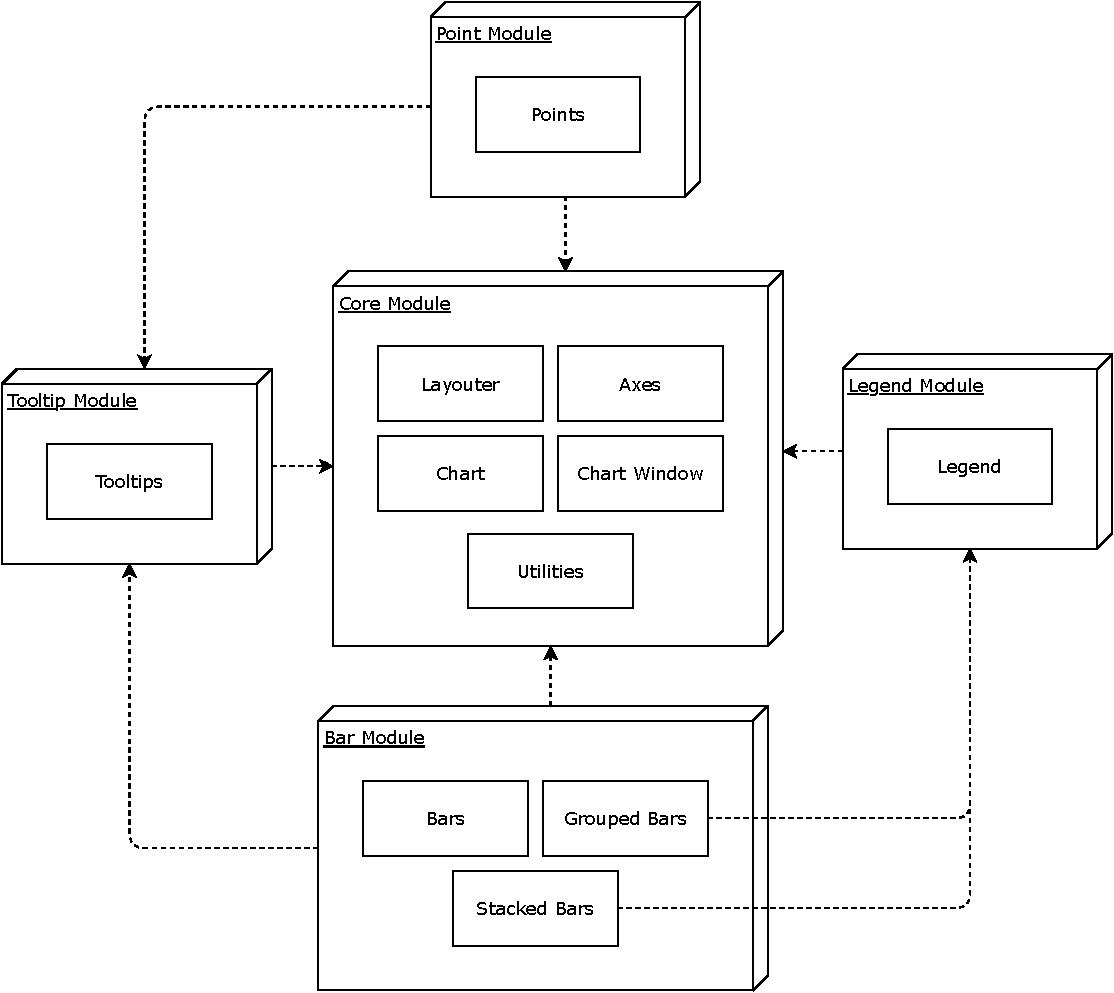
\includegraphics[keepaspectratio,width=\linewidth,height=\fullh]{diagrams/respvis-modules.pdf}
  \caption[Modules of RespVis]{
    This diagram shows the different modules of the RespVis library.
    It also shows the most important submodules contained in the individual modules.
    The directional arrows connecting modules indicate dependencies between them.
    \imgcredit{Image created by the author of this thesis using \href{https://www.diagrams.net/}{diagrams.net}.}
  }
  \label{fig:Modules}
\end{figure}


\section{Core Module}

The core module contains the necessary core functionality of the library.
It is the base module that all other modules depend on and includes various utility functions, the layouter, axes, chart base components, and chart window base components.
RespVis heavily relies on utility functions to reuse and structure recurring operations.
The core module contains utilities to deal with arrays, elements, selections, and texts, as well as geometric utilities that simplify the handling of positions, sizes, rectangles, circles, and paths.
The layouter is a custom component that enables controlling the layout of SVG elements with CSS.
% It achieves this by replicating the DOM tree of SVG elements that should be layed out with HTML \code{<div>} elements, applying the appropriate CSS configuration on the replicated elements, and storing their calculated layout information on the original SVG elements.
% Render functions can then use the stored layout information on layed out SVG elements to render their content so that it fits within the corresponding boundaries. 
Axis components have been included in the core module because they are important components that occur in nearly every visualization.
% However, since only cartesian charts have been implemented thus far, only cartesian axes can be found in the implementation.
Lastly, the chart and chart window components provide base functionalities that simplify the creation of more specialized charts and chart windows.
The core module implementation is located in the \code{src/lib/core/} directory of the project.

\subsection{Utilities}

The utilities provided by RespVis are split on multiple modules that are placed in the \code{utilities/} directory of the core module.
These modules include types and functions that perform array, element, selection and text operations as well as modules that simplify geometric operations with positions, sizes, rectangles, circles and paths.
Utility functions are grouped into modules by the type of entity they operate on.
This grouping is also reflected in the names of functions, which all begin with the type of entity a function is associated with.

\TODO{Capitalize "core module", "array utility module", ... ?}
Array utilities can be found in the \code{utilities/array.ts} module.
The \code{Array} class in the JavaScript base implementation already offers a wide variety of convenient methods to work with arrays.
These methods form a solid foundation that allows handling of a broad range of situations.
However, not everything is covered out of the box and some things require manual implementations, which is why the RespVis library offers additional functions that simplify commonly encountered tasks.
The \code{arrayEquals} function is used to verify equality of two arrays and also works if they contain nested arrays within them.
Type guard functions are used to determine the type of a variable at runtime.
For this purpose, two different array type guard functions are provided in the array utility module: \code{arrayIs}, which evaluates to true if the passed parameter is an array, and \code{arrayIs2D}, which evaluates to true if the passed parameter is a two-dimensional array.
The \code{arrayIs} function is merely a wrapper around the \code{Array.isArray} method.
Theoretically, the \code{Array.isArray} method could be used directly instead of the \code{arrayIs} function, but because the \code{arrayIs2D} function is required, the \code{arrayIs} function has also been added for consistency reasons.
The last function in the array utility module is the \code{arrayPartition} function.
This function receives an array and a partition size as parameters and returns a partitioned version of the input array with each chunk containing the number of items specified by the partition size parameter.


% elementRelativeBounds
% elementComputedStyleWithoutDefaults
% elementSVGPresentationAttrs

The element utilities module located at \code{utilities/elements.ts} in the core module contains functions and constants related to document elements.
The \code{elementRelativeBounds} function is used to calculate the bounding box of an element relative to the bounding box of its parent in viewport coordinates.
Internally, it uses the \code{getBoundingClientRect} function, which returns the actual bounding box of an element in viewport coordinates and, as opposed to other ways of accessing an element's position, it also takes transformations into account.
Every element has a set of CSS styles applied on them and the \code{Window.getComputedStyle} method can be used to access the active style of an element.
The style declaration object returned by this method contains all possible CSS properties and their values, regardless of whether or not they are set to default values.
Sometimes this behavior may be desired, but in this library, the computed style is used during the preparation of a downloadable SVG document to transform styles set in CSS to attributes on the individual elements.
If every possible style property on every element would be mapped to an attribute, the resulting SVG document would be unnecessarily bloated because only those properties that are not set to their default values actually have an effect.
For this reason, the \code{elementComputedStyleWithoutDefaults} function has been implemented to calculate the computed style of an element and remove all properties that are set to default values from the returned style declaration object.
This is implemented by adding a \code{<style-dummy>} element as a sibling of the element of interest, getting the computed styles of both elements, and calculating the difference between them.
To speed up these calculations, the \code{elementComputedStyleWithoutDefaults} function accepts an array of property names as its second parameter and will only consider the properties listed in this array.
The constant \code{elementSVGPresentationAttrs} array contains all names of the presentation attributes listed in the SVG 1.1 specification \parencite{SVG11}.
Since only these SVG attributes can be styled via CSS, only these properties need to be taken into account when preparing downloadable SVG documents.

% Transition default type variables
% Selection default type variables
% SelectionOrTransition default type variables
% Selection.attr add possible null return value
% Selection.dispatch allow Partial parameters
% isSelection
% isTransition

\TODO{When to write \code{Selection} and when to write Selection? What about plural? \code{Selections} or \code{Selection}s?}
Selection utilities are implemented in the \code{utilities/selection.ts} module.
They include typing improvements for the D3 \code{Selection}, \code{Transition}, and \code{SelectionOrTransition} interfaces and type guards to distinguish between \code{Selection}s and \code{Transition}s.
The \code{Selection}, \code{Transition}, and \code{SelectionOrTransition} interfaces allow the specification of four different type variables: the type of elements contained in the \code{Selection} or \code{Transition}, the type of data that is bound to those elements, the type of the parents of those elements, and the type of data that is bound to those parents.
In most cases, the type variables related to parent elements do not influence the logic of code using these interfaces and could be omitted to keep it more concise.
For this reason, these interface have been reexported with default types set on all of the type variables.
This means that whenever type variables need to be manually specified, only those that need to be set to specific types need to be explicitly stated.
Further typing improvements have been made to the \code{attr} and \code{dispatch} methods of the \code{Selection} interface.
The D3 type declarations of the \code{Selection.attr} method do not include \code{null} as a possible return value.
This is wrong because this method will actually result in a \code{null} value when reading an attribute that does not exist.
To fix this inconsistency and catch potential bugs related to this during compilation, the type declaration of the \code{Selection.attr} method has been overwritten in the Selection utility module to also include \code{null} as a possible return value.
A less important but nonetheless convenient improvement has been made to the type declaration of the \code{Selection.dispatch} method.
This method allows the dispatching of custom events with certain parameters that control different aspects of how this event is dispatched and the data that may be bound to it.
In practice, not all parameters need to be specified at every invocation because the implementation of the \code{Selection.dispatch} method will provide default values for all of them.
However, this is not reflected in the type declaration of the function, which requires every parameter to be provided every time the function is called.
To fix this, the Selection utility module provides a type declaration overwrite for the \code{Selection.dispatch} function that wraps the type of the parameters parameter into the \code{Partial} type.
Apart from these typing improvements, this module also provides the \code{isSelection} and \code{isTransition} type guard functions that are used to distiguish between \code{Selection}s and \code{Transition}s.


Utilities for dealing with \code{<text>} elements can be found in the \code{utilities/text.ts} module.
It contains rather basic functionalities that simply set specific data attributes to specific values on \code{<text>} elements.
The text utility module holds functions that set data attributes controlling the horizontal and vertical alignment of \code{<text>} elements, as well as their orientation.
Horizontal and vertical alignment is configured using the \code{textAlignHorizontal} and \code{textAlignVertical} functions.
These functions respectively set the \code{data-align-h} and \code{data-align-v} attribute on a Selection or Transition to the value passed into either function as a string enum parameter of type \code{HorizontalAlignment} or \code{VerticalAlignment}.
The \code{HorizontalAlignment} enum represents the string values \code{\"left\"}, \code{\"center\"} and \code{\"right\"}, while the \code{VerticalAlignment} enum represents the values \code{\"top\"}, \code{\"center\"} and \code{\"bottom\"}.
The distinct \code{data-align-h} and \code{data-align-v} attribute values are then used in the \code{respvis.css} file to declare different \code{text-anchor} and \code{dominant-baseline} values that control the alignment of \code{<text>} elements.
Text orientation is set using the \code{textOrientation} function.
This function sets the \code{data-orientation} attribute on a Selection or Transition to the value specified via the string enum parameter of type \code{Orientation}.
The \code{Orientation} enum represents the values \code{\"horizontal\"} and \code{\"vertical\"}.
These \code{data-orientation} attribute values are then used in CSS to set the \code{text-anchor}, \code{dominant-baseline}, and \code{transform} properties of a \code{<text>} element, in order to rotate it accordingly and position it correctly inside the bounding box calculated by the layouter.


% Position interface
% positionRound
% positionEquals
% positionToString
% positionFromString
% positionToAttrs (SelOrTrans)
% positionFromAttrs (SelOrTrans)
% positionToTransformAttr (SelOrTrans)

The core module also contains utilities that simplify geometric operations.
One of these utilities is the position utility module located at \code{utilities/position.ts}.
This module contains the \code{Position} interface and various functions to perform operations related to it.
The \code{Position} interface consists of the \code{x} and \code{y} number members.
Rounding these members is necessary to be able to correctly compare equality of two \code{Position}s and to not render unnecessarily long strings when transforming them into string representations.
This rounding is performed with the \code{positionRound} function, which allows the specification of the number of decimals the members variables should be rounded to.
Equality comparision between two \code{Position} variables can be performed with the \code{positionEquals} function, which evaluates to \code{true} if both \code{Position}s are equal and \code{false} if not.
To transform a \code{Position} into its string representation of the form \code{\"x, y\"}, the \code{positionToString} function can be used.
Its counterpart, the \code{positionFromString} function, can be used to transform a string in the correct format into a \code{Position}.
A large part of RespVis consists of modifying the attributes of elements.
Therefore, the \code{positionToAttrs} function can be used to set the \code{x} and \code{y} attributes of a \code{SelectionOrTransition} to the values of the \code{x} and \code{y} members of a \code{Position}.
Similarly, the \code{positionToTransformAttr} function can be used to set the \code{transform} attribute of a \code{SelectionOrTransition} to a translation representing a \code{Position}.
The position utility module also contains the \code{positionFromAttrs} function, which can be used to create a \code{Position} from the \code{x} and \code{y} attributes of a \code{SelectionOrTransition}.

% Size
% sizeRound
% sizeEquals
% sizeToString
% sizeFromString
% sizeToAttrs
% sizeFromAttrs

The size utility module is located at \code{utilities/size.ts} in the core module is very similar to the position utility module.
It contains the \code{Size} interface, which consists of the \code{width} and \code{height} number member variables.
The \code{sizeRound} function is used to round the member variables of a \code{Size} object to a certain number of decimals.
To compare two \code{Size} objects for equality, the \code{sizeEquals} function can be used.
Similar to the equivalent functions in the position utility module, the \code{sizeToString} and \code{sizeFromString} functions can be used to convert between \code{Size} objects and their string representations.
Moreover, the \code{sizeToAttrs} can be used to set the \code{width} and \code{height} attributes of a \code{SelectionOrTransition} to the values of a \code{Position} object and the \code{sizeFromAttrs} function can be used to create a new \code{Position} object from the values of these attributes.

% Rect
% rectRound
% rectEquals
% rectToString
% rectFromString
% rectToAttrs
% rectMinimized
% rectFitStroke
% rectPosition
% rectCenter
% rectLeft, rectRight, rectTop, rectBottom
% rectTopLeft, rectTopRight, rightBottomRight, rightBottomLeft

Utilities for dealing with rectangles can be found in the rectangle utility module, which is located under \code{utilities/rect.ts} in the core module.
This module contains the \code{Rect} interface, which is the union of the \code{Position} and \code{Size} interfaces and therefore describes an object with the number member variables \code{x}, \code{y}, \code{width}, and \code{height}.
Similar to the position and size utility modules, this module contains the \code{rectRound} function to round \code{Rect} objects, the \code{rectEquals} function to compare two of them for equality, the \code{rectToString} and \code{rectFromString} functions to convert between \code{Rect} objects and their string representations, and the \code{rectToAttrs} and \code{rectFromAttrs} functions to convert between objects and \code{x}, \code{y}, \code{width}, and \code{height} attributes.
Since the \code{Rect} interface is a combination of the \code{Position} and \code{Size} interfaces, most of the functions in this module internally use the functions provided by the position and size utility modules.
The \code{rectMinimized} function is used in transitions that grow or shrink a \code{<rect>} element from or to their center.
It creates a minimized version of the passed \code{Rect}, which is infinitely small and positioned at the original \code{Rect}'s center.
When declaring a stroke for SVG elements, it is drawn exactly on the outline of an element's silhouette.
This means that a stroke will extend outside the original bounds of an element by half the stroke width, which can lead to unwanted artefacts like the stroke of bars in a bar chart overlapping over the chart's axes.
To counteract this, the \code{rectFitStroke} function is provided to adjust the bounding box of \code{Rect} objects to account for a stroke of a certain width around them.
Lastly, the rectangle utility module provides functions to calculate specific positions inside of rectangles.
The most generic of these functions is the \code{rectPosition} functions.
This function enables the calculation of a position inside of a rectangle via a two-dimensional parameter that expresses a position as the percental width and height distance from a rectangle's top-left corner.
All other position-calculating rectangle utility functions are simply shorthand functions that internally call the \code{rectPosition} function.
The \code{rectCenter} function returns a \code{Position} object representing the center position of a \code{Rect} object.
The \code{rectLeft}, \code{rectRight}, \code{rectTop}, and \code{rectBottom} functions return \code{Position} objects that represent the middle position of a \code{Rect} object's edges.
Similarly, The \code{rectTopLeft}, \code{rectTopRight}, \code{rectBottomRight}, \code{rectBottomLeft} functions can be used to calculate the corner positions of a rectangle.

% Circle
% circleRound
% circleEquals
% circleToString
% circleFromString
% circleToAttrs
% circleFromAttrs
% circleMinimized
% circleFitStroke
% circlePosition
% circleInsideRect
% circleOutsideRect

The last geometric primitive whose handling is simplified by a RespVis utility module is a circle.
The circle utility module can be found at \code{utilities/circle.ts} in the core module.
It contains the \code{Circle} interface, which describes a circle object as a \code{center} property of type \code{Position} and a \code{radius} property of type \code{number}.
This module also contains equivalent functions to those found in previously mentioned utility modules: \code{circleRound}, \code{circleEquals}, \code{circleToString}, \code{circleFromString}, \code{circleToAttrs}, \code{circleFromAttrs}, \code{circleMinimized}, and \code{circleFitStroke}.
Furthermore, the \code{circlePosition} function can be used to calculate positions using an angle that defines the direction and an optional parameter that defines the distance from the circle's center as a percentage of the circle's radius.
The circle utility module also contains functions to create circles from rectangles.
These functions are the \code{circleInsideRect} function to calculate the largest circle that can fit inside of a rectangle and the \code{circleOutsideRect} function to calculate the smallest circle that encloses a rectangle.

% pathRect
% pathCircle

The purpose of the path utility module is to provide functions that simplify the creation of path definitions that can be set on \code{<path>} elements.
It is located at \code{utilities/path.ts} in the core module and only contains a small number of functions.
The \code{pathRect} function creates a path definition that represents a rectangle. 
A \code{<path>} element with a path definition representing a rectangle can be used instead of a \code{<rect>} element. 
Similarly, the \code{pathCircle} function creates a path definition that represents a circle.
Such a path definition is used on a \code{<path>} element to render a circle instead of using a \code{<circle>} element.
The reason for using \code{<path>} elements rather than more descriptive shape elements is that path elements can change their shape dynamically without replacing elements.
Since only the \code{d} attribute of a path needs to change when the path's shape is altered, it is also possible to smoothly transition between shapes by interpolating the path definition strings.

\subsection{Layouter}

The Layouter is the most novel contribution of this work.
It is a component that is wrapped around an SVG document and allows to configure the layout of elements in this document with CSS.
Instead of implementing a custom layout algorithm, the Layouter builds on layout engines integrated in browsers, which have already been summarized in Section~\ref{sec:BrowserEngines}.
Earlier proof of concept implementations used the FaberJS \parencite{FaberJS} and Yoga \parencite{Yoga} layout engines to calculate layouts, but these implementations were not further pursued because they limited layouting to either Grid or Flexbox-based constraints.
Furthermore, the use of already existing browser functionality in the current implementation leads to a reduced bundle size and to visualization authors being able to use all the layouting capabilities natively offered by browsers.

CSS has always been the foundation of responsive web design for HTML-based websites because of its ability to adapt the presentation of elements and the possibility of defining different presentations for different contexts via media queries.
A large part of the responsive power that CSS offers comes from its ability to change the positioning and layout of elements.
As already mentioned in previous chapters, CSS can be used to style certain aspects of SVG documents, but it is not possible to use CSS layouting techniques to position SVG elements.
Even though there are already other visualization libraries such as Chartist \parencite{Chartist} and Highcharts \parencite{Highcharts} that allow the use of CSS to style visualizations, none of them offer the possibility to modify the layout of visualizations via CSS.
This means that visualization authors have to learn and use custom APIs to position elements, which limits the range of possible layouts to those supported by the individual libraries. 

The Layouter distinguishes between laid-out and non-laid-out elements because not every element in a visualization profits from being laid out by it. 
Laid-out elements are elements whose position and size are being calculated by the Layouter, whereas non-laid-out elements are ignored during the layout process. 
Theoretically, the layouter could be used to position all elements of a visualization since it is only necessary to determine a good mapping that maps a rectangular bounding box to the desired SVG shape for each element.
However, the positioning of elements in a visualization is constrained more strictly than the positioning of elements in typical HTML documents.
The content of a visualization is communicated more through visual features such as position, size, and shape of elements rather than simply through text which can be positioned much more freely.  
For this reason, many elements of a visualization must be positioned at specific locations with specific dimensions, which means there is very little profit in laying them out with an elaborate layout algorithm.
These exactly-positioned elements like the \code{<rect>} elements of bar series and the \code{<circle>} elements of point series are usually positioned directly via their SVG attributes.
Positioning them via the Layouter would be rather pointless and only cause unnecessary overhead.

The layout process can be seen in Figure~\ref{fig:LayoutProcess} and consists of three phases that have been implemented in the \code{layouterCompute} function:
\begin{enumerate}
\item Replication:
The structure of the SVG document that shall be laid out must be replicated with HTML \code{<div>} elements. These elements are referred to as \enquote{layout elements} and they have the same classes and \code{data-*} attributes as the original SVG elements they are replicating.
This replication of the SVG document with HTML documents is necessary because CSS-based positioning can only affect HTML elements.

\item Layout:
The replicated layout elements are affected by CSS rules that configure their positioning and are automatically laid out by browsers. 
If the Selectors of CSS rules used to style SVG elements only select them using classes and \code{data-*} attributes, the layout of these elements can be directly configured in these rules because they will also be applied to the corresponding layout elements.

\item Synchronization:
The positions of the layout elements are synchronized with their respective SVG elements.
This means that the calculated bounding boxes of layout elements are set as \code{bounds} attributes on SVG elements, which can be used in subsequent renderings.
In addition to that, the Layouter sets different default attributes on different types of SVG elements that aim to represent the boundaries of individual elements.
\end{enumerate}

\begin{figure}[tp]
\centering
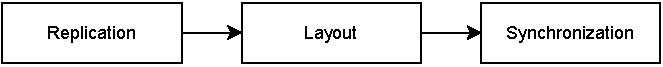
\includegraphics[keepaspectratio,width=\linewidth,height=\fullh]{diagrams/respvis-layout-process.pdf}
\caption[Layout Process of the Layouter]{
  This diagram shows the three phases of the layout process of the RespVis Layouter. 
  During the replication phase, the SVG document that shall be laid out is replicated with HTML \code{<div>} elements. 
  Afterward, these HTML elements are laid out by the browser in the layout phase, and the positions of the laid-out HTML elements are applied to their respective SVG elements during the synchronization phase.
  \imgcredit{Image created by the author of this thesis using \href{https://www.diagrams.net/}{diagrams.net}.}
}
\label{fig:LayoutProcess}
\end{figure}


During the replication process, the structure of an SVG document is replicated with HTML \code{<div>} elements. 
This replication was implemented using a hierarchical D3 data join in which the original SVG elements are bound as data objects to layout elements.
This hierarchical data join results in a counterpart in the hierarchy of layout elements for each SVG element that should be affected by the layouter.
Since not every SVG element should be positioned via the Layouter, the Layouter must know which to ignore.
For this, the \code{data-ignore-layout} and \code{data-ignore-layout-children} attributes have been introduced.
Elements that have the \code{data-ignore-layout} attribute or are children of elements that have the \code{data-ignore-layout-children} attribute will not be replicated.

To configure the layout of layout elements in CSS, it must be possible to select them uniquely with a CSS Selector.
This Selector should be as similar as possible to the Selector of the original SVG element to make it as easy as possible to configure the CSS properties of layout elements.
For this purpose, the class attributes and all data-* attributes of SVG elements are copied to their corresponding layout elements.
In addition to the classes of the replicated SVG element, the layout class is set on all layout elements.
By doing this, it is possible to specifically select the layout element of an SVG element via the same Selector by adding the layout class to the same Selector. 
If CSS rules of SVG elements use only classes and data attributes in their Selectors, the properties of corresponding layout elements can directly be configured in the same rules.
An example of how the replicated layout element tree of an SVG document looks can be seen in Listing~\ref{list:LayouterStructure}.
Furthermore, an example of CSS rules that set various properties of SVG elements and their layout elements can be seen in Listing~\ref{list:LayouterCSS}.  

\begin{samepage}
\lstinputlisting[%
  float=tp,
  aboveskip=\floatsep,
  belowskip=\floatsep,
  xleftmargin=0cm,              % no extra margins for floats
  xrightmargin=0cm,             % no extra margins for floats
  %
  basicstyle=\footnotesize\ttfamily,
  frame=shadowbox,
  numbers=left,
  label=list:LayouterStructure,
  caption={[Replicated Layout Structure of an SVG Document]%
    The replicated layout element structure of an SVG document.
    Every SVG element has a corresponding layout element that has the same classes and \code{data-*} attributes.
    In addition to the classes of the original SVG element, every layout element also has the \code{layout} class to allow specific targeting of layout elements via CSS Selectors.
  },
]{listings/layouter-structure.html}
\end{samepage}

\begin{samepage}
\lstinputlisting[%
  float=tp,
  aboveskip=\floatsep,
  belowskip=\floatsep,
  xleftmargin=0cm,              % no extra margins for floats
  xrightmargin=0cm,             % no extra margins for floats
  %
  basicstyle=\footnotesize\ttfamily,
  frame=shadowbox,
  numbers=left,
  label=list:LayouterCSS,
  caption={[CSS Rules to Style SVG]%
    These CSS rules are used to configure the layout and style of an SVG document that is being laid out by the Layouter.
    Since the Selectors of these CSS rules only use \code{class} and \code{data-*} attributes to match elements, the same rule can be used to configure the properties of an SVG element and its corresponding layout element.  
    The structure of the SVG document and its replicated layout elements can be seen in Listing~\ref{list:LayouterStructure}.
  },
]{listings/layouter-css.css}
\end{samepage}

The size of dynamically-sized elements depends on the size of their content.
Since layout elements exist separately from their SVG elements and can not access their content, a manual solution had to be implemented that sets the size of layout elements to the content size of their SVG elements when required.
An example of dynamically-sized elements is \code{<text>} elements because their size is rarely declared in absolute units and usually depends on the size of their text contents. 
The custom \code{--fit-width} and \code{--fit-height} CSS properties were introduced to activate the manual copying of dimensions from SVG elements to their layout elements. 
These boolean properties can be set in CSS rules and are being checked during the replication phase via the \code{window.getComputedStyle} method.
If at least one of these properties is set to true, the dimensions of the SVG element are calculated with the \code{Element.getBoundingClientRect} method and respectively set as \code{width} or \code{height} properties of the \code{style} attribute on the corresponding layout element.
By doing this, layout elements will have the same size as their svg elements and can be properly used in the calculation of the overall layout. 

Layout elements are automatically laid out by the browser during the layout phase of the layout process. 
Since the layout elements are simply \code{<div>} elements that have been styled in CSS rules, the browser can position them automatically via its integrated layout engine.
This positioning happens as soon as the layout elements have been rendered.
After this, the final bounding boxes of layout elements can be calculated and used for further operations.  

In the synchronization phase of the layout process, the Layouter iterates over all the layout elements, calculates their bounding boxes, and set this boundary information as attributes on the corresponding SVG elements.
Bounding boxes of layout elements are calculated relative to their parent elements using the \code{elementRelativeBounds} utility function.
This bounding box is then converted to its string representation via the \code{rectToString} utility function and set as the \code{bounds} attribute on the corresponding SVG elements. \TODO{Rename bounds attr to data-bounds}
The \code{bounds} attribute can then be deserialized to a \code{Rect} object whenever the bounding box of an SVG element is needed in subsequent renderings of SVG components. 
In addition to setting the \code{bounds} attribute of SVG elements, the Layouter also sets specific attributes on different types of SVG elements that make them fit into their calculated bounding boxes.
These attributes can, of course, be overwritten in later renderings, but they represent sensible defaults that express the boundaries of laid-out elements.
If the Layouter would not set these default attributes, they would have to be set manually on every laid-out element during the rendering process, which would be less convenient and lead to duplicated code in various places.
For SVG elements that can be mapped directly to rectangular areas, such as \code{<svg>} and \code{<rect>} elements, the Layouter sets the \code{x}, \code{y}, \code{width}, and \code{height} attributes to the values of their bounding boxes.
SVG shape elements that have explicit sizes and positions but are not rectangular, such as \code{<circle>} and \code{<line>} elements, also receive attributes that make them fit into their boundaries. 
Other SVG elements that are not explicitly sized, such as \code{<g>} and \code{<text>} elements, are merely moved to the correct position by setting their \code{transform} attribute to a translation so that their top-left corners aligns with the top-left corners of their bounding boxes. 
The Layouter does not automatically recalculate the dimensions of exactly-positioned elements based on the changed dimensions of the composite \code{<svg>} or \code{<g>} element containing them.
This has to be manually implemented in the render functions of the various components.

Using the Layouter requires a more complex rendering process than would be needed if the boundaries of elements would already be known before rendering them.
The way the Layouter works, some elements need to be rendered before calculating the layout, and afterward, when the positions and sizes of all elements are known, the visualization needs to be rendered in its final form. 
This visualization rendering process when using the Layouter consists of three phases and is shown in Figure~\ref{fig:RenderProcess}.
The three phases of the render process are the first rendering phase to render elements affecting the layout, the layouting phase, and the second rendering phase to render elements affected by the layout.
In the first rendering phase, all elements and attributes that affect the layout of a visualization need to be rendered.
This mostly includes laid-out container \code{<svg>} and \code{<g>} elements that contain exactly-positioned child elements, but it also means that the contents of dynamically-sized elements, such as \code{<text>} elements and axes, need to be fully rendered in this phase too.
The layouting phase is where all the operations of the already-described layout process are being performed.
During this phase, the bounding boxes of laid-out elements are calculated and persisted as attributes that can be accessed during the second rendering phase.
In the second rendering phase, the desired bounding box position and size of every element is known and can be used to perform a second rendering of the complete visualization.
Here, every element affected by the layout, which is every element, is rendered at its final position with its final dimensions.
In theory, the first and second rendering phases of components could be implemented in separate functions.
However, it is more convenient to invoke the same render function twice and perform some operations only if the appropriate \code{bounds} attribute has already been set.


\begin{figure}[tp]
\centering
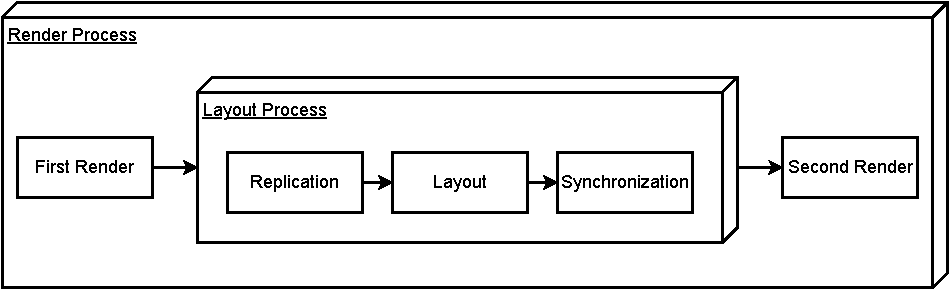
\includegraphics[keepaspectratio,width=\linewidth,height=\fullh]{diagrams/respvis-render-process.pdf}
\caption[Render Process When Using the Layouter]{
  This diagram shows the three phases of the render process when using the RespVis Layouter. 
  During the first render phase, every element that affects the layout needs to be rendered.
  The layout phase of the render process is equivalent to the layout process described in Figure~\ref{fig:LayoutProcess}.
  In this phase, the Layouter calculates the final positions and sizes of laid-out elements and stores them as attributes on the SVG elements.
  During the second render phase, all elements of the visualization are rendered at their final positions with their final dimensions by using the boundary information calculated in the layout phase.
  \imgcredit{Image created by the author of this thesis using \href{https://www.diagrams.net/}{diagrams.net}.}
}
\label{fig:RenderProcess}
\end{figure}


\subsection{Axes}

% axisData
%   scale
%   title
%     orientation
%   subtitle
%     orientation
%   configureAxis
%     d3 axis
%   default values
% axisRender
%   structure
%     .title (dynamically sized wh)
%     .subtitle (dynamically sized wh)
%     .ticks-transform (dynamically sized w or h) warum?
%       .ticks
%     laid out with CSS Grid
%   d3 axis function to render ticks
%     delete attributes and use data attributes and css to configure presentation of axis
% axisBottomRender
%   .axis-bottom
%   CSS grid with 3 rows and 1 full width column
%   title and subtitle orientations
%   tick text alignment
% axisLeftRender
%   .axis-left
%   CSS grid with 3 columns and 1 full height row
%   title and subtitle orientations
%   tick text alignment

achsen werden verwendet um scales, welche das mapping von abstrakten werten auf zwei-dimensionale positionen representieren, zu visualisieren.
Die implementierung aller verfuegbaren Achsen komponenten kann in der \code{axis.ts} datei im core module gefunden werden.
momentan werden von der RespVis library nur kartesische achsen zur verfuegung gestellt da bislang nur kartesische charts implementiert wurden.
diese kartesischen achsen komponenten werden per ihrer position relativ zu der draw area einer visualisierung unterschieden und zum aktuellen zeitpunkt wurden nur left and bottom axis components in der RespVis library implementiert.
Dies sind die mit abstand am haeufigsten angetroffenen positionierungen von kartesischen achsen und wurden gewaehlt, da mit ihnen die meisten use cases abgedeckt werden koennen. 
Eine achse besteht aus ticks, welche die eigentliche visualisierung einer scale sind, und aus einem optionalen titel und untertitel, welche gerendert werden koennen um die konfiguration der visualisierten scale zusaetzlich zu beschreiben. 
Ein Beispiel dafuer wie eine gerenderte left und bottom axis aussehen koennte, kann in Figure~\ref{fig:Axes} gesehen werden. 

\begin{figure}[tp]
\centering
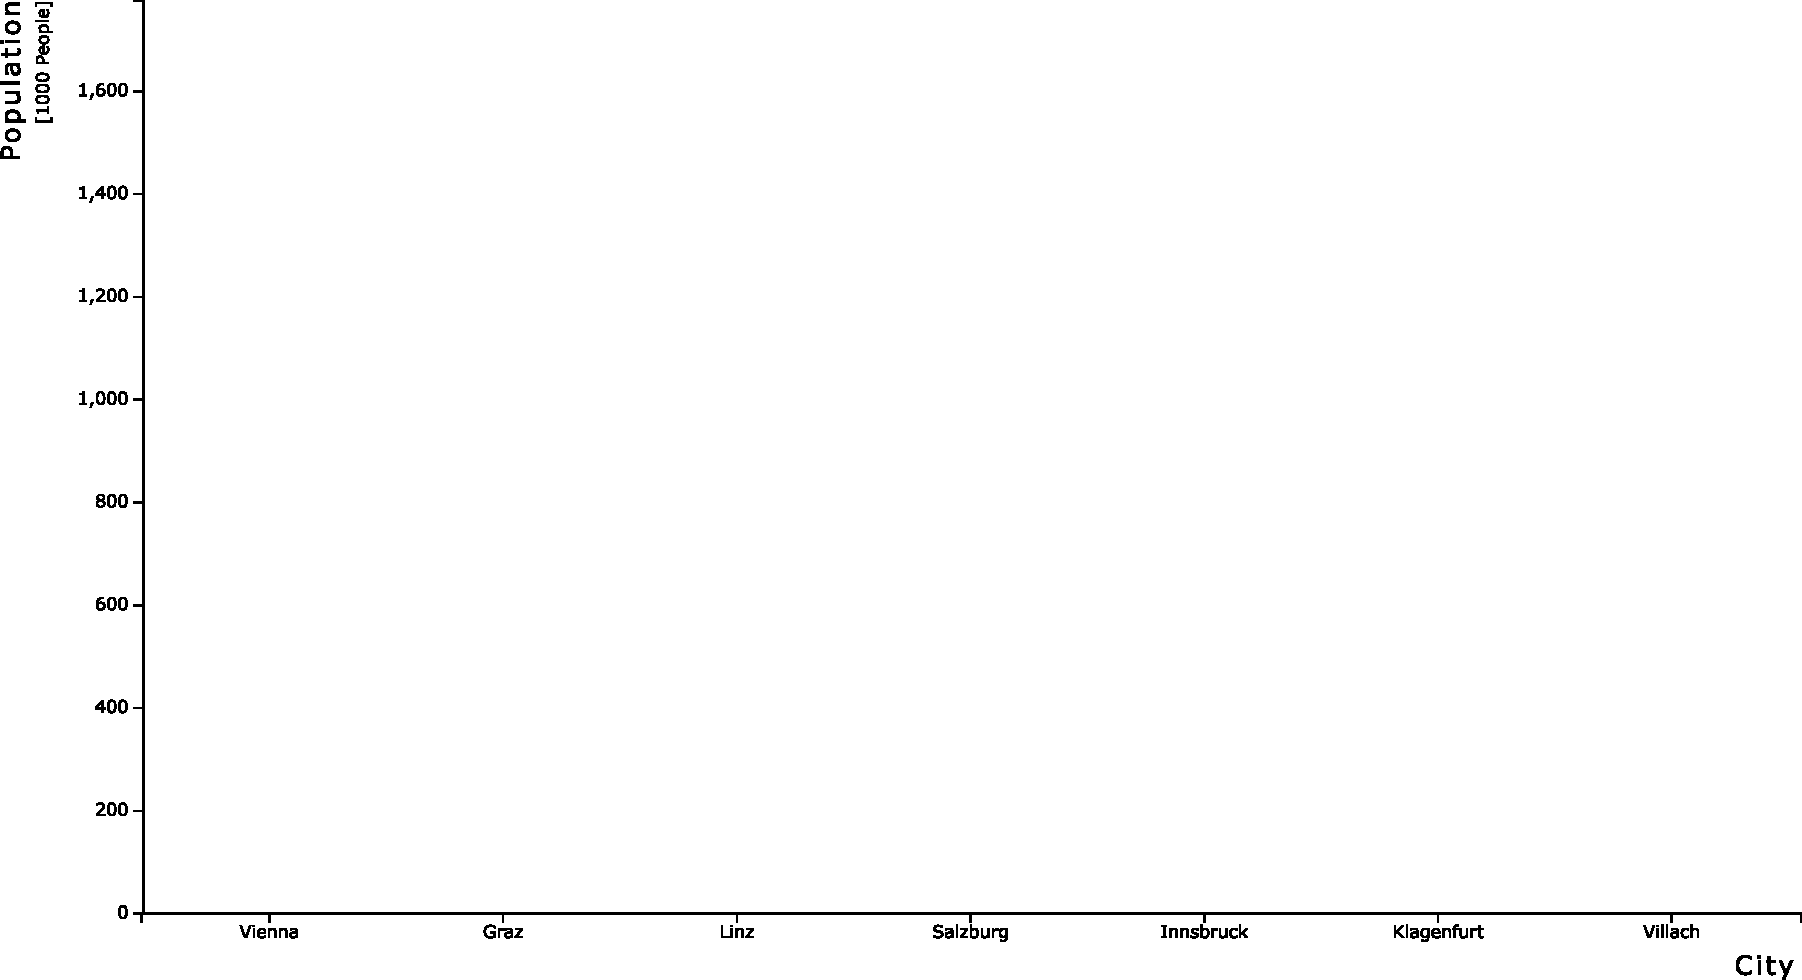
\includegraphics[keepaspectratio,width=\linewidth,height=\fullh]{diagrams/axes.pdf}
\caption[RespVis Axis Components]{
  This figure shows how a rendered left and bottom axis may look like.
  The left axis consists of a title, subtitle, and ticks, whereas the bottom axis only consists of ticks and a title. 
  \imgcredit{Image created by the author of this thesis using RespVis and \href{https://inkscape.org/}{Inkscape}.}
}
\label{fig:Axes}
\end{figure}
  

Das \code{Axis} interface beschreibt die shape eines data objects mit welchem das rendering einer achse konfiguriert werden kann.
Es beinhaltet ein \code{scale} property, welches die scale representiert die visualisiert werden soll, die \code{title} und \code{subtitle} string properties, und das \code{configureAxis} function property, welches verwendet werden kann um die darunterliegende D3 axis zu konfigurieren bevor sie rendered wird.  
wie auch die meisten anderen komponenten bestehen auch achsen komponenten hauptsaechlich aus zwei funktionen: einer data creation funktion und einer render funktion.
die \code{axisData} funktion wird verwendet um ein data object in der form des \code{Axis} interfaces zu erzeugen.
sie wird mit einem \code{Partial<Axis>} object als parameter aufgerufen und liefert ein neues object bei dem alle nicht-gesetzten aber benoetigten properties des parameter objektes mit standardwerten befuellt wurden.
die \code{axisBottomRender} und \code{axisLeftRender} funktionen werden verwendet um eine left oder bottom axis in einem composite element zu rendern auf welchem eine achse mittels eines gebundenen \code{Axis} data object konfiguriert wurde. 
diese beiden render functions verwenden die nicht-exportierte \code{axisRender} base function um duplizierten code zu vermeiden.
alle achsen haben die selbe struktur von elementen und werden so viel wie moeglich ueber CSS positioniert und gestyled.
Der root einer achse ist ein CSS Grid container und definiert das layout der title, subtitle und ticks elemente.
Die standardkonfiguration einer left axis positioniert diese elemente in einem three-column layout in welchem die title, subtitle und ticks elemente in dieser reihenfolge von links nach rechts plaziert werden.
Bei einer bottom axis sieht die standardkonfiguration eine positionierung derselben elemente in einem three-row layout vor in welchem die ticks, title und subtitle elemente in dieser reihenfolge von oben nach unten plaziert werden.
Weiters werden die title und subtitle elemente einer left axis mittels der \code{textOrientation} utility function vertikal orientiert um horizontalen platz zu sparen.
Die RespVis achsen komponenten verwenden intern jeweils die \code{axisBottom} und \code{axisLeft} funktionen aus dem D3 axis module \parencite{D3Axis} um die ticks einer achse zu rendern.
da diese D3 funktionen attributes verwenden um die einzelnen elemente der ticks einer achse zu positionieren und zu stylen, muessen diese attributes direkt nachdem die ticks gerendert wurden soweit es geht entfernt werden um die konfiguration via CSS zu ermoeglichen. 

\subsection{Chart}

% chart
% chart cartesian

\subsection{Chart Window}

% chart window
% menu dropdown
% series checkbox
% tool filter nominal
% tool download svg
% resize event dispatcher

\section{Legend Module}

\section{Tooltip Module}

\section{Bar Module}

\subsection{Basic Bars}

\subsection{Grouped Bars}

\subsection{Stacked Bars}

\section{Point Module}